\newpage

\section{Remerciements}\label{remerciements}

\bigskip

Je tiens tout d'abord à remercier Benjamin Tierny et Robin Komiwes pour
m'avoir permis d'effectuer mon stage au sein de leur entreprise puis de
m'avoir proposé de prolonger cette expérience.

\bigskip

Je remercie également Julien Iguchi-Cartigny pour l'aide qu'il m'a
apporté en tant que tuteur universitaire.

\bigskip

Samy Meftali, mes enseignants et tout le personnel de l'Université de
Lille 1 pour la qualité de la formation qu'ils proposent.

\bigskip

Pour finir j'aimerais remercier toute l'équipe de \emph{Dernier Cri}
pour m'avoir aidé aussi souvent à étendre mes compétences.

\newpage

\section{Introduction}\label{introduction}

\bigskip

Dernier Cri est une Start-Up crée en 2011 axée vers l'innovation
digitale. L'équipe est en charge du développement, du déploiement et de
la maintenance d'applications pour le compte de plusieurs clients. Ces
applications sont hébergées chez des fournisseurs de plateforme (PaaS)
ou d'infrastructure (IaaS).

\bigskip

L'entreprise ne disposant pas d'administrateur système, ma mission en
son sein consiste à maintenir l'infrastructure utilisée ainsi qu'à être
force de proposition pour améliorer celle-ci. Dans ce but, je suis amené
à prendre en main et à gérer les différents services souscrit par
l'entreprise ainsi qu'à répondre aux demandes des clients au sujet de
l'infrastructure.

\bigskip

Mon stage chez Dernier Cri vise donc à proposer différents mécanismes
d'automatisation de tâches d'administration de façon à restreindre les
interventions de développeur au niveau du système. Cela permet de gagner
en maintenabilité et en vitesse de déploiement. Dans cette optique, je
suis amené à déveloper un \emph{Chatops}, un outil d'administration
d'infrastructure par la discussion qui associé à \emph{Ansible}, un
programme d'orchestration de machines, offre une très grande réactivité
en cas de panne et une gestion efficace de l'infrastructure.

\newpage

\section{Contexte du stage}\label{contexte-du-stage}

\bigskip

\begin{figure}[htbp]
\centering
\includegraphics{logo_DC}
\caption{logo}
\end{figure}

\bigskip

\emph{\href{http://derniercri.io}{Dernier Cri}}, anciennement
\emph{Nectify}, est une société d'innovation digitale fondée en 2011 par
Benjamin Tierny et Robin Komiwes. À ses débuts, \emph{Nectify} s'est
concentré sur le développement de \emph{\href{http://fre.sc}{Fresc}}, un
outil de partage d'avis sur des visuels. Par la suite l'activité de
l'entreprise s'est étendu à la prestation de services centrée sur
l'innovation puis plus récemment au \emph{Big Data} pour devenir. Cette
évolution dans les services proposées a motivé le changement de nom pour
devenir \emph{Dernier Cri}.

\bigskip

\emph{Dernier Cri} met un point d'honneur à proposer à ses clients une
solution complète adaptée à un problème spécifique. De la conception à
la réalisation, l'entreprise accompagne ses clients de A à Z pour
aboutir à un produit au plus proche des besoins de ceux-ci. Cela permet
aux développeurs d'opérer dans différents domaines d'activités et
d'avoir une vue globale du développement de produit.

\newpage

\section{Analyse de l'existant}\label{analyse-de-lexistant}

\bigskip

\subsection{Services}\label{services}

\bigskip

Dernier Cri développe des applications pour ses clients et en assure le
déploiement continu ainsi que la maintenance. L'entreprise fait appel à
plusieurs \emph{SaaS} \emph{(Software as a Service)} pour l'aider dans
certaines tâches comme la gestion de \emph{logs} ou l'analyse de code.
Ces informations doivent être centralisées et accessibles à l'ensemble
de l'équipe, pour cela nous utilisons les intégrations Slack de ces
services, de cette manière nous sommes en mesure d'accéder à ces
informations en temps réél.

\bigskip

Actuellement ces intégrations consistent uniquement en des rapports
envoyés à intervalle réguliers, tandis qu'il faudrait que vous soyons en
mesure de les obtenir à la demande pour pouvoir corriger une panne le
plus rapidement possible.

\newpage

\subsection{Infrastructure}\label{infrastructure}

\bigskip

\subsubsection{Serveurs}\label{serveurs}

\bigskip

Nous faisons appel à des \emph{IaaS} \emph{(Infrastructure as a
Service)} pour héberger notre infrastructure, ainsi nous profitons de
fiabilité et de performances accrues pour nos serveurs. Nous gérons
également les noms de domaines pour le compte de nos clients afin qu'ils
n'aient pas à s'en soucier.

\bigskip

Le manque d'homogénéité dans l'infrastructure la rend compliquée à
maintenir, en effet les serveurs sont hébergés chez 3 fournisseurs
différents (\emph{Rackspace}, \emph{OVH},
\href{http://digitalocean.com}{\emph{Digital Ocean}}) et les noms de
domaines sont gérés par 2 services différents : \emph{Gandi} pour
l'achat et la gestion de certains domaines,
\href{http://cloudfare.com}{\emph{Cloudfare}} pour la gestion des
autres. Il s'agit là de quelques exemples de ce qui rend
l'infrastructure difficile à maintenir.

\subsubsection{Docker}\label{docker}

\bigskip

L'utilisation faite de \emph{docker} pose aussi quelques problèmes. Les
conteneurs ne sont pas indépendant ni réutilisable, chacun embarque un
serveur SSH pour pouvoir démarrer l'application ce qui devrait être fait
au démarrage du conteneur.

\bigskip

De plus, les conteneurs contiennent plusieurs services ce qui les rend
difficilement réutilisable car trop spécifiques à une application. Il
faudrait disposer de conteneurs générique qui pourraient être
réutilisable facilement par plusieurs applications, par exemple la
plupart des applications utilisent un serveur \emph{Redis} dont
l'installation est faite directement dans le conteneur principal. Nous
devrions disposer d'un conteneur \emph{Redis} générique prêt à l'emploi
pour chaque application.

\newpage

\section{Objectifs du stage}\label{objectifs-du-stage}

\bigskip

L'objectif de mon stage consiste à apporter mon soutien à la gestion de
l'infrastructure, en réduisant le nombre de services proposant les mêmes
fonctionnalités. Je prend également en charge la gestion
d'infrastructure et configure les serveurs pour chaque nouvelles
application produite par l'entreprise. Cela m'a amené à revoir
l'utilisation de \emph{Docker} chez \emph{Dernier Cri} afin d'en
améliorer l'efficacité.

\bigskip

Je suis également force de proposition pour faire évoluer
l'infrastructure afin de gagner en autonomie et en efficacité, dans ce
but j'ai mis en place \emph{Ansible}, un orchestrateur de serveurs afin
d'automatiser les tâches d'administration les plus communes comme la
configuration de serveurs ou le déploiement d'applications.

\bigskip

J'ai également pu développer un \emph{chatops}, un outil
d'administration système via la conversation. Intégré au \emph{Slack} de
l'entreprise, il permet à tout le personnel d'obtenir des informations
sur un serveur ou une application et d'effectuer des résolutions simples
en cas de panne. De plus, en s'appuyant sur \emph{Ansible} et sur un
système de plugins, le \emph{Chatops} est une solution générique qui
peut facilement s'adapter à l'évolution de notre infrastructure.

\bigskip

En complément des tâches précédentes, j'ai l'opportunité de réaliser du
développement pour divers projets ce qui me permet de comprendre
davantage le travail de développeur et m'aide à apporter de meilleures
solutions d'automatisation.

\newpage

\section{Ansible}\label{ansible}

\bigskip

\subsection{Présentation}\label{pruxe9sentation}

\bigskip

\begin{quote}
Ansible is a radically simple IT automation engine that automates cloud
provisioning, configuration management, application deployment,
intra-service orchestration, and many other IT needs.
\emph{(\href{https://www.ansible.com/how-ansible-works}{source})}
\end{quote}

\bigskip

Ansible est un outil d'automatisation et d'administration très puissant.
Il s'agit d'un serveur léger permettant d'aggréger plusieurs machines
(\emph{noeuds}) et d'exécuter sur celles-ci des programmes
(\emph{modules}). Le seul prérequis est de disposer d'un point d'accès à
ces noeuds.

\bigskip

Il s'agit d'un client léger, il n'est pas nécessaire de l'installer sur
un serveur, un simple poste client suffit car l'ensemble des commandes
sont exécutées via un protocole de communication, le plus souvent
\emph{SSH}. Le résultat d'une commande est également très lisible.

\bigskip

Voici un exemple d'utilisation d'ansible pour vérifier qu'une machine
répond :

\begin{Shaded}
\begin{Highlighting}[]
\NormalTok{$ }\KeywordTok{ansible} \NormalTok{-i hosts -m ping ssh-test}
\KeywordTok{ssh-test} \KeywordTok{|} \KeywordTok{SUCCESS} \NormalTok{=}\KeywordTok{>} \NormalTok{\{}
    \StringTok{"changed"}\NormalTok{: }\KeywordTok{false}\NormalTok{,}
    \StringTok{"ping"}\NormalTok{: }\StringTok{"pong"}
\NormalTok{\}}
\end{Highlighting}
\end{Shaded}

\newpage

\subsection{Configuration}\label{configuration}

\bigskip

Ansible permet de gérer une infrastructure hétéroclite de manière
transparente en s'appuyant sur la puissance de protocoles de
communication tels que \emph{SSH}.

\bigskip

Il est très facile de configurer \emph{Ansible} pour qu'il ait accès à
un grand nombre de machines. Sur les serveurs il suffit d'ajouter la clé
d'accès du serveur \emph{Ansible}. Il est parfois nécessaire de
configurer les règles \emph{sudo} pour qu'\emph{Ansible} puisse exécuter
certaines commandes.

\bigskip

Du côté client, il s'agit d'un fichier de configuration qui permet de
regrouper les machines disposant de caractéristiques communes. Ainsi il
est possible de créer un groupe \emph{cassandra} qui vous permettra
d'exécuter les tâches de maintenance et de mise à jour liées à
l'ensemble de vos noeuds. Un serveur peut appartenir à plusieurs groupes
ce qui permet de configuer des groupes pour chaque type de technologies
utilisées

\newpage

\subsection{Modules}\label{modules}

\bigskip

Il existe beaucoup de modules pour Ansible. Ceux-ci permettent de gérer
tout les aspects d'administration système et il existe également des
modules correspondant à un grand de nombre de services tels
qu'\emph{AWS} ou \emph{Digital Ocean}.

\bigskip

Il est par exemple possible d'écrire un script générique pour créer une
machine chez \emph{Digital Ocean} et la configurer afin qu'elle soit
prête à l'utilisation le plus vite possible. L'utilisation des groupes
évoqués précédemment permettront ensuite d'y installer les dépendances
nécessaires.

\bigskip

Ces modules sont très bien documentés et offrent une couche
d'abstraction supplémentaires sur la gestion d'arguments pour éviter les
problèmes de compréhension. Il est de plus possible, si nécessaire,
d'écrire soi-même un module correspondant à un besoin spécifique.

\newpage

\subsection{Playbooks}\label{playbooks}

\bigskip

La véritable puissance d'Ansible réside dans la possibilité d'écrire des
scripts (\emph{playbooks}) permettant d'exécuter une série de tâches sur
un ou plusieurs noeuds de votre architecture, chaque tâche correspondant
à un module.

\bigskip

Ci-dessous, un exemple de playbook ansible installant git via
\emph{apt}.

\begin{Shaded}
\begin{Highlighting}[]
\CommentTok{# ping.yml}

\KeywordTok{-} \FunctionTok{hosts:} \NormalTok{ssh-test}
  \FunctionTok{tasks:}
    \KeywordTok{-} \FunctionTok{name:} \NormalTok{Install Git}
      \FunctionTok{become:} \NormalTok{yes}
      \FunctionTok{apt:} \NormalTok{name=git update_cache=yes}
\end{Highlighting}
\end{Shaded}

And the return of \emph{ansible-playbook} command

\bigskip

\begin{Shaded}
\begin{Highlighting}[]
\KeywordTok{PLAY} \NormalTok{**********************************************************}

\KeywordTok{TASK} \NormalTok{[setup] **************************************************}
\KeywordTok{ok}\NormalTok{: [ssh-test]}

\KeywordTok{TASK} \NormalTok{[Ping the given hosts] ***********************************}
\KeywordTok{changed}\NormalTok{: [ssh-test]}

\KeywordTok{PLAY} \NormalTok{RECAP ****************************************************}
\KeywordTok{ssh-test}       \NormalTok{: ok=2    changed=1    unreachable=0    failed=0   }
\end{Highlighting}
\end{Shaded}

\bigskip

Les playbboks disposent de multiples fonctionnalités permettant
d'automatiser toute sorte de traitement. Il est par exemple possible de
définir des variables dans un playbook ou directement dans la définition
d'un noeud pour pouvoir utiliser des scripts génériques.

\newpage

\subsection{Ansible chez Dernier Cri}\label{ansible-chez-dernier-cri}

\bigskip

L'utilisation d'Ansible au sein de Dernier Cri permet une gestion de
l'infrastructure plus claire et plus efficace. La gestion des serveurs
et des applications est presque intégralement reléguée à Ansible, ce qui
facilite les tâches d'administration système. L'écriture de playbooks
génériques rend très facile la création de nouvelles machines, leur
configuration et l'installation des dépendances spécifiques pour le
déploiement. D'autre playbooks permettront ensuite de maintenir ces
machines et d'y déployer une nouvelle version d'une application.

\bigskip

Un autre avantage d'Ansible a été de réduire les accès sur chacune des
machines. En effet il était auparavant nécessaire d'ajouter manuellement
les clé d'accès \emph{SSH} sur chacune des machines nouvellement créées.
Ce processus a amené des problèmes de sécurité, il devenait compliqué de
savoir qui disposait d'accès sur quelle machine et certaines anciennes
clés était toujours présente dans l'infrastructure.

\bigskip

Grâce à ansible, il est devenu possible de créer une machine supervisant
les autres. Ce superviseur gérant l'ensemble des machines de
l'infrastructure, celles-ci ne devant disposer que de la clé d'accès du
superviseur pour être configurées. La gestion des droits d'accès des
différents utilisateurs a donc été réduite à la configuration d'une
seule machine, assurant ainsi la scalabilité de l'infrastructure

\bigskip

Pour complèter l'usage d'Ansible, nous mettons également en place un
\emph{Chatops} qui permet d'appeler ces scripts directement via le Slack
de l'entreprise. Cela nous permet non seulement de pouvoir gérer
l'infrastructure directement depuis un smartphone mais cela garantit
aussi une certaine sécurité en réduisant les accès directs aux serveurs
qui seront uniquement effectuées par le \emph{Bot}.

\newpage

\section{Chatops}\label{chatops}

\bigskip

\subsection{Présentation}\label{pruxe9sentation-1}

\bigskip

Le chatops est un programme connecté au \emph{Slack} de l'entreprise et
couplé à l'infrastructure Ansible permettant de réaliser différentes
tâches d'administration système. Il se présente sous la forme d'un
utilisateur comme les autres au sein du chat et interagira avec les
utilisateurs par le biais de commandes.

\bigskip

Par exemple voici la fonction d'aide intégrée au chatops :

\begin{figure}[htbp]
\centering
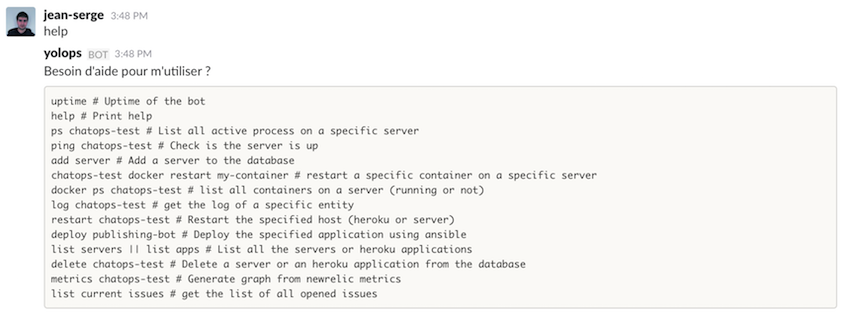
\includegraphics{help.png}
\caption{help}
\end{figure}

\bigskip

Le chatops a pour but de faciliter les tâches de déploiement et de
maintenance des applications, en effet il leur suffit maintenant de
saisir des commandes simplifiées dans le canal approprié pour obtenir
les informations qui leur sont nécessaires. Le chatops est également
capable d'effectuer un diagnostic simple de l'état d'une machine et
tentera de résoudre les problèmes.

\newpage

\subsection{Fonctionnement}\label{fonctionnement}

\bigskip

Le chatops fonctionne de manière assez simple, il s'agit d'un programme
Node.JS qui se connecte à l'API temps réél de Slack via un Token qui lui
est donné. Une fois connecté, le bot recevra tout les messages envoyés
dans un channel auquel il appartient, s'il reconnait une commande parmis
ces messages, il exécutera la fonction qui lui est associée.

\bigskip

Le format des commandes implémentées est volontairement simplifié afin
que même les personnes n'ayant pas de connaissances en informatique
soient capable de les comprendre et de les utiliser. \bigskip

Les commandes sont écrites sous forme de plugins de façon à être
configurable et réutilisable, elles peuvent être divisées en 2
catégories : la collecte d'informations et l'exécution de playbooks.

\newpage

\subsubsection{Collecte d'informations}\label{collecte-dinformations}

\bigskip

La collecte d'information se traduit par une requête vers l'API de l'un
des services utilisé chez Dernier Cri. Cela permet de centraliser les
informations concernant un serveur ou une application au sein d'un même
canal de communication. Cela s'avère utile en cas de panne, les
développeurs peuvent directement sur le chat les informations nécessaire
à la résolution du problème telles que les logs de l'application ou
l'état de la machine.

\begin{figure}[htbp]
\centering
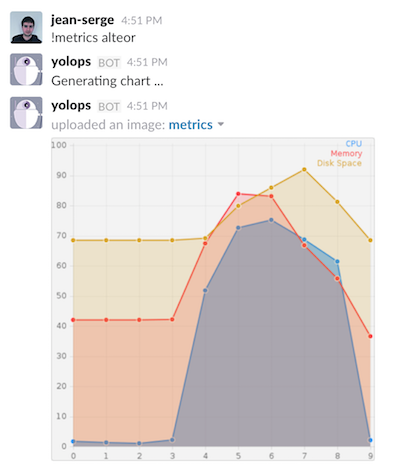
\includegraphics{metrics.png}
\caption{metrics}
\end{figure}

\newpage

\subsubsection{Le Chatops et Ansible}\label{le-chatops-et-ansible}

\bigskip

L'exécution de playbooks Ansible permet d'agir sur l'infrastructure sans
pour autant devoir s'y connecter directement, cela offre une réactivité
plus grande et permet de faciliter la résolution d'un problème sans
nécessairement disposer de compétences en administration système.
L'utilisation de playbook spécifiques à une application permettra de
réduire son temps de déploiement sans pour autant augmenter la charge de
travail des développeurs.

\begin{figure}[htbp]
\centering
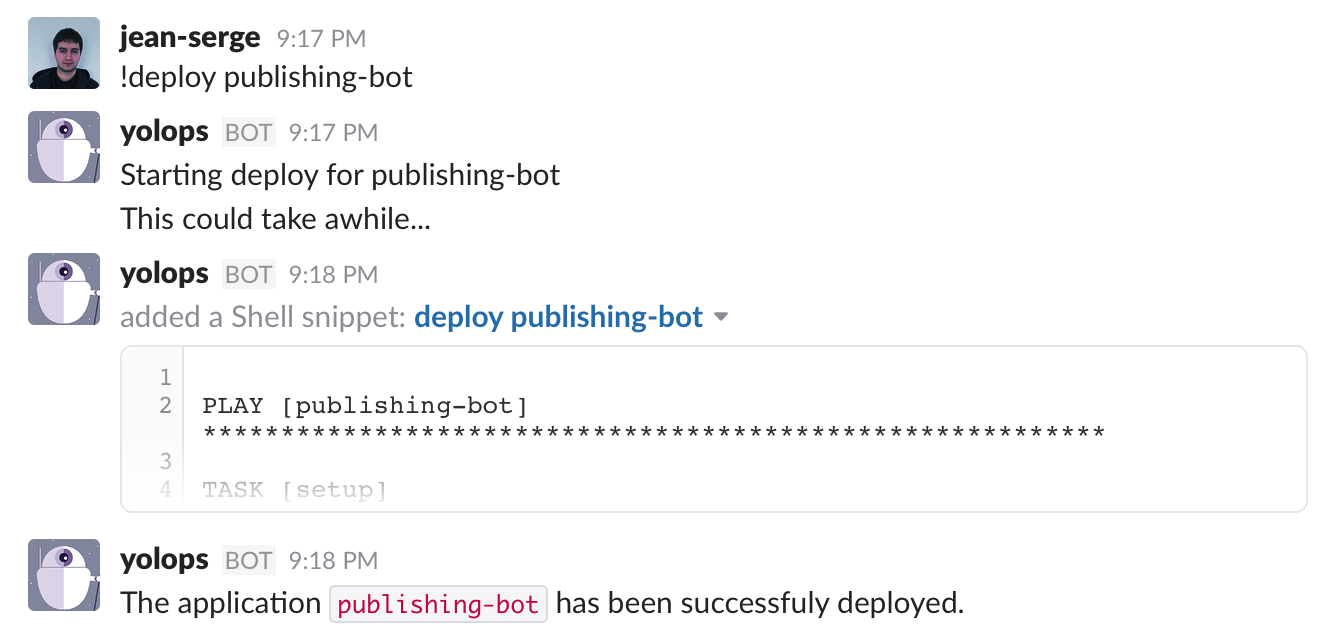
\includegraphics{deploy.png}
\caption{}
\end{figure}

\newpage

\subsection{Le Chatops chez Dernier
Cri}\label{le-chatops-chez-dernier-cri}

\bigskip

Le chatops nous permet d'être plus réactif et efficace en cas de
problème, il est désormais possible d'obtenir l'ensemble des
informations nécessaires à la résolution d'une panne directement au sein
du \emph{Slack} professionnel. De plus tout les développeurs peuvent
l'utiliser sans pour autant connaitre les commandes d'administration
système à exécuter.

\bigskip

Il représente un gain de temps pour les développeurs en facilitant le
déploiement ou la maintenance d'applications. Il n'est plus nécessaire
de se connecter au serveur et de retrouver la ou les commandes à
exécuter, il suffit de le demander au chatops.

\newpage

\section{Autres travaux}\label{autres-travaux}

\bigskip

Durant ce stage j'ai eu l'opportunité de participer à des tâches
variées, allant de l'administration système au développement
d'applications. Cela m'a permis de me familiariser avec de nouvelles
technologies telles que \emph{Ruby} ou \emph{Node.JS} mais également de
renforcer mes compétences dans certains domaines tels que les script
\emph{bash} ou le multi-processing \emph{python}.

\subsection{Administration système}\label{administration-systuxe8me}

\bigskip

Au sein de \emph{Dernier Cri} j'ai le rôle d'administrateur système, je
suis en charge de la gestion de l'infrastructure qu'il s'agisse de
serveurs, des services externes en passant par la gestion des noms de
domaine et des certificats. Ces responsabilités m'ont permis de prendre
conscience des nombreux aspects à prendre en compte avant même le
développement d'une application web.

\bigskip

Je suis également amené à revoir l'utilisation de \emph{docker} au sein
de l'entreprise, celle-ci est maladroite et peut être amélioré. Les
conteneurs actuels contiennent systématiquement un serveur \emph{SSH}
indépendant pour pouvoir démarrer l'application conteneurisée ce qui
consomme des ressources inutilement. Pour corriger cela il suffit de
rédiger un script qui sera exécuté au démarrage du conteneur, de cette
manière il n'est plus nécessaire de se connecter au conteneur pour
démarrer l'application.

\bigskip

Les images utilisées peuvent aussi être allégées en réécrivant le
\emph{Dockerfile} utilisé et en y retirant les fichiers inutiles (cache,
doc, \ldots{}). De plus il convient généralement de n'inclure qu'un seul
service par \emph{Docker} ce qui est plus sécurisé mais surtout
réutilisable. Certains services sont actuellement inclus dans plusieurs
conteneur alors qu'il suffirait de créer une image indépendante et de
l'utiliser lors du déploiement.

\newpage

\subsection{Développement}\label{duxe9veloppement}

\bigskip

J'ai pu travailler sur un projet en \emph{python} effectuant un grand
nombre de requêtes API suivi d'un traitement sur la réponde de celle-ci.
Le nombre de requêtes étant élevée et les informations récupérées
n'étant pas inter-dépendantes j'ai écrit un programme créant 8
sous-processus réalisant cette tâche.

\bigskip

Suite au \emph{Chatops} j'ai eu l'occasion de travailler sur d'autre
\emph{bots}, un \emph{chatbot} et le \emph{publishing-bot}.

\bigskip

Le \emph{chatbot} est semblable au \emph{chatops} mais a pour but
d'exécuter des tâches internes à l'entreprise telles que la saisie des
temps ou les réservations de local et de matériel.

\bigskip

Le \emph{publishing-bot} est un \emph{bot} écrit en \emph{Ruby} capable
de convertir un répertoire Github sous forme de PDF, d'HTML ou d'Epub
puis de le publier. Ce bot est utilisé pour publier les documents de
l'entreprise puis, grâce au \emph{chatbot}, d'envoyer un message sur le
\emph{Slack} de l'entreprise indiquant l'URL pour accéder à ces
documents.

\newpage

\section{Conclusion}\label{conclusion}

\bigskip

La mise en place d'Ansible et du Chatops chez Dernier Cri est un premier
pas vers l'automatisation de l'infrastructure. Actuellement certaines
application sont encore inadaptée à ce système, l'objectif sur le long
terme est donc de les rendre compatible en révisant leur méthode de
déploiement et de maintenance.

\bigskip

Mon prochain objectif au sein de Dernier Cri est d'apporter mon soutien
dans l'amélioration de l'infrastructure Docker de l'entreprise, celle-ci
est en effet assez simpliste est pourrait être revue afin de faciliter
le déploiement d'application mais aussi la préparation d'environnement
de développement. Cela a déjà été mit en place sur certaines
applications et je souhaite poursuivre cette tendance.

\bigskip

Sur le plus long terme j'espère apporter davantage de mécanismes
d'automatisation à \emph{Dernier Cri} pour rendre le déploiement
d'application le plus rapide et simple possible.
